Em \cite{Razinkova2014}, foi proposto um controlador PD para a descrição adequada das trajetórias definidas de um helicóptero quadrotor \textit{Indoor}. Para permitir um funcionamento adequado \textit{Outdoor}, foi integrado ao controlador PD um controle adaptativo, adicionando termos ao controlador convencional, de forma a permitir o ajuste correto da trajetória do quadrotor quando submetido a distúrbios nos eixos X e Y (plano horizontal). Os resultados mostraram que o controlador adaptativo melhorou consideravelmente o controle de trajetória do drone, reduzindo em 64\% o erro de posicionamento para os casos de trajetória em linha reta ao longo do plano XY, e em 72\% para os casos de trajetória circular sobre o plano XY. Segundo os autores, este resultado representa uma melhora significativa, uma vez que o controlador resultante possui uma arquitetura simples e não requer computação extensiva, o que é indesejado para qualquer controle de sistema, especialmente para UAVs, devido à sua bateria limitada.

Em \cite{Mustapa2014} é proposto um controlador PID para efetuar o controle sobre a estabilidade da altitude de um helicóptero quadrotor. Neste trabalho, foi utilizado um modelo matemático desenvolvido previamente para descrever o comportamento de um quadrotor. Para ajustar os parâmetros do controlador PID, foi necessário realizar um experimento para determinar o momento de inércia do drone. O sistema utilizado para tanto foi o de pêndulo bifiliar. Uma vez levantados os valores necessários, um controlador PID foi ajustado e se mostrou eficiente. A simulação do sistema se deu no Mat-lab Simulink.

\citeonline{Khatoon2014} também propuseram um controlador PID para controlar a estabilidade em altitude de um drone, mantendo a posição no eixo XY constante, mesmo esta altitude sendo uma variável muito sensível a mudanças em outros parâmetros. No trabalho, é mostrado que um controlador PID sozinho é capaz de exercer tal controle com robustez. A escolha deste controlador se deu graças à sua robustez e facilidade de modelagem. Entretanto, é também apontado pelos autores que, apesar da simplicidade para se modelar um controlador PID, isto requer uma modelagem do sistema como um todo, o que não é fácil, devido à sua estrutura complexa, suas dinâmicas não lineares e sua natureza subatuada. O sistema modelado para o drone mostrou ser altamente instável, justificando a necessidade de um controlador. A partir de extensivas simulações no MATLAB/Simulink, o sistema desenvolvido se mostrou bem sucedido, implementando, de fato, um controle robusto de altitude para um helicóptero quadrotor.

\subsection{Métodos de Controle Inteligente de Helicópteros Quadrotores}
\label{sec:trab-rel-quadrotores-sub-ia}

Além das técnicas de controle tradicionais, encontram-se também na literatura diversas abordagens para a construção de controladores de estabilidade para \textit{drones} utilizando técnicas da Inteligência Computacional. 

As propostas vão do uso de algoritmos de otimização (e.g.\ algoritmos genéticos, PSO) ao uso de neuro-fuzzy expandido para o espaço dos números complexos.

%22
%\cite{Rezazadeh2013}
Em \cite{Rezazadeh2013}, é proposto um controlador neuro-fuzzy (ANFIS) para controlar a estabilidade em altitude de um UAV. O módulo fuzzy acoplado a um controlador PID é usado para controlar cada atitude (i.e.\ cada um dos ângulos). Os controladores fuzzy atualizam os ganhos do controlador PID \textit{online} para produzir uma resposta apropriada. De fato, o módulo fuzzy produz ganhos proporcional e derivativo. O ganho integral é setado como um fator do ganho derivativo. A taxa desses ganhos é determinado posteriormente através de otimização multi-objetivo, usando um algoritmo genético sem elitismo. O controlador neuro-fuzzy usado para controlar a estabilidade de um quadricóptero é mostrado na \autoref{fig:Rezazadeh2013_estrutura_anfis}, sendo esta a estrutura típica de uma arquitetura ANFIS para um sistema com duas entradas e uma saída.
%O esquema do controlador é mostrado na \autoref{fig:Rezazadeh2013_diagrama_controlador}.
\iffalse
\begin{figure}[!htb]
    \centering
    \caption{Diagrama em blocos do controlador Fuzzy PID proposto em \cite{Rezazadeh2013}}
    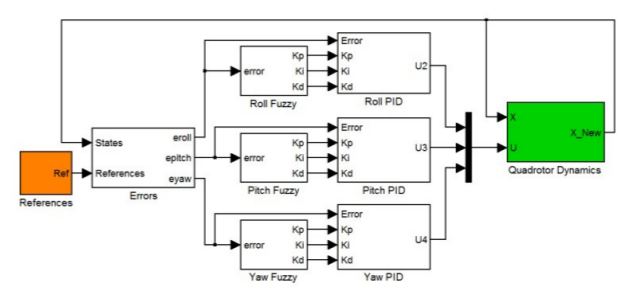
\includegraphics[width=0.7\textwidth]{./04-figuras/Rezazadeh2013_diagrama_controlador}
    \fonte{\cite{Rezazadeh2013}}
    \label{fig:Rezazadeh2013_diagrama_controlador}
\end{figure}
\fi

\begin{figure}[!htb]
    \centering
    \caption{Estrutura do ANFIS multicamadas de duas entradas e uma saída}
    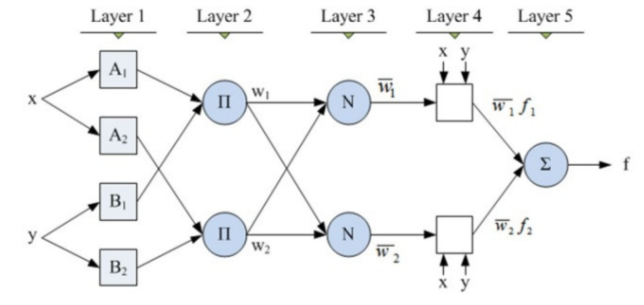
\includegraphics[width=0.7\textwidth]{./04-figuras/Rezazadeh2013_estrutura_anfis}
    \fonte{\cite{Rezazadeh2013}}
    \label{fig:Rezazadeh2013_estrutura_anfis}
\end{figure}

Como se pode ver pela \autoref{fig:Rezazadeh2013_estrutura_anfis}, a saída é calculada diretamente pelo ajuste dos pesos das entradas de acordo com as regras de inferência fuzzy. Estas regras, que são a base de conhecimento, são determinadas por um algoritmo computacional baseado em redes neurais \cite{Rezazadeh2013}. O controlador proposto foi comparado a um simples controlador PID e, a partir de simulações, foi mostrado que obteve melhor resposta, por exemplo, sobre o tempo de assentamento e a sobrelevação. Outro resultado obtido foi de que o controlador ANFIS é capaz de estabilizar o sistema quando exposto a perturbações externas.

%34
%\cite{Mahfouz2013}
Em \cite{Mahfouz2013}, foi proposto um controlador parecido. Neste trabalho, também foi sugerido um controlador ANFIS que, juntamente a um algoritmo genético, ajusta os pesos de um controlador PID. Mais uma vez, o controlador desenvolvido obteve sucesso, sendo apto a garantir a estabilidade de um drone mesmo quando sujeito a condições externas. No trabalho, foi mostrado que a sobrelevação do controlador ANFIS é melhor do que a do PID. Além disto, o erro do estado estável no caso do ANFIS é zero, enquanto o erro do estado estável no caso do controaldor PID não é efetivamente zero. Uma conclusão muito importante a que se chega é: do ponto de vista de robustez, os dois controladores são robustos; do ponto de vista de performance, o ANFIS é melhor que o PID.


%14
%\cite{Maj2013}
Em \cite{Maj2013} é proposto um controle de estabilidade para um quadricóptero usando lógica fuzzy. Neste trabalho, três controladores fuzzy são usados: um para cada um dos dois eixos horizontais e mais um controlador geral para todo o sistema. O controlador foi desenvolvido para operar sobre um Arduino. O erro angular e a aceleração são as variáveis linguísticas. Em ambos os casos, são usados cinco termos linguísticos: muito negativo (NL), pouco negativo (NS), zero (Z), pouco positivo (PS) e muito positivo (PL). Os conjuntos NS, Z e PS são triangulares enquanto os conjuntos NL e PL são trapezoidais, como mostra a figura \autoref{fig:Maj2013_fuzzy_sets}. 

\begin{figure}[!htb]
    \centering
    \caption{Conjuntos fuzzy usados em \cite{Maj2013}; a) erro de posição; b) erro de giro }
    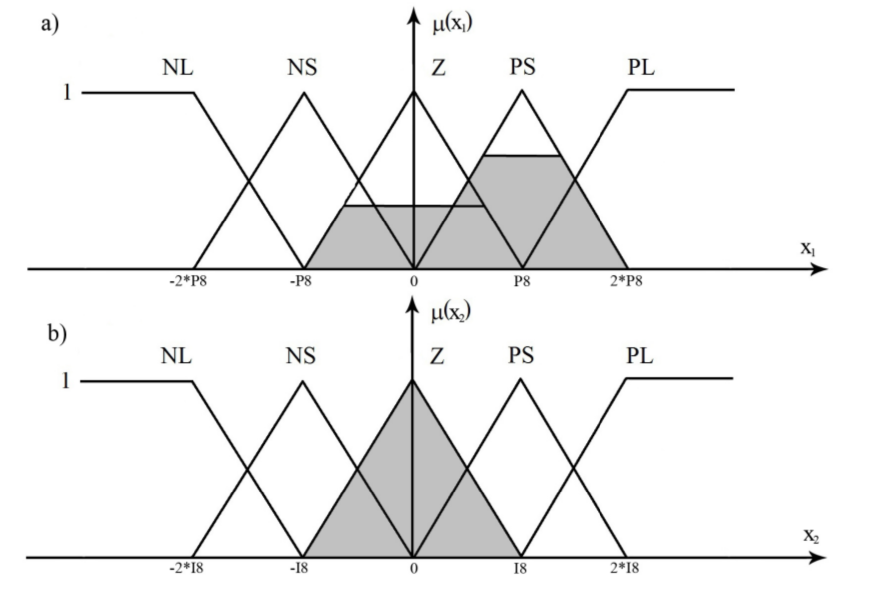
\includegraphics[width=0.6\textwidth]{./04-figuras/Maj2013_fuzzy_sets}
    \fonte{\cite{Maj2013}}
    \label{fig:Maj2013_fuzzy_sets}
\end{figure}

O bloco de fuzzificação calcula o grau de confiança dos conjuntos de entrada. Um segundo bloco executa a inferência, que calcula o grau de confiança dos conjuntos de saída. Como operadores AND e OR para os conjuntos fuzzy, são usados respectivamente as operações MIN e MAX. Como o controlador fuzzy é do tipo PD e este tipo de controlador não fornece uma posição zero, um bloco adicional é usado para controlar a integral do erro de posição. O resultado é, portanto, um controlador híbrido. Entretanto, os autores propõem também uma solução para substituir o bloco integrador por um bloco contendo três conjuntos fuzzy: negativo, neutro e positivo. Como resultado, obtém-se um \textit{array} tridimencional com setenta e cinco regras, ao invés das vinte e cinco obtidas no caso de usar o bloco integrador. O \autoref{qua:Maj2013_table_rules_inference} mostra as vinte e cinco regras de inferência fuzzy usadas no controlador proposto com bloco integral.

\begin{quadro}[!htb]
    \centering
    \caption{Regras de inferência fuzzy usadas em \cite{Maj2013}\label{qua:Maj2013_table_rules_inference}}
    % \begin{tabular}{|p{3cm}|p{3cm}|p{3cm}|p{3cm}|p{3cm}|p{3cm}|}
    \begin{tabular}{c|c|c|c|c|c|}
        \cline{2-6}
        & \multicolumn{5}{c|}{\textbf{Erro de Giro}} \\
        
        \hline
        \multicolumn{1}{ |c| }{\textbf{Erro Angular}} & 
                            \textbf{NL} &
                            \textbf{NS} & 
                            \textbf{Z}  & 
                            \textbf{PS} & 
                            \textbf{PL}  \\
        \hline
        \multicolumn{1}{ |c| }{\textbf{NL}} & 
                            PL &
                            PL & 
                            PL & 
                            PS & 
                            Z  \\
        \hline
        \multicolumn{1}{ |c| }{\textbf{NS}} & 
                            PL &
                            PL & 
                            PS & 
                            Z  & 
                            NS \\

        \hline
        \multicolumn{1}{ |c| }{\textbf{Z}} & 
                            PL &
                            PS & 
                            Z  & 
                            NS & 
                            NL \\
        \hline
        \multicolumn{1}{ |c| }{\textbf{PS}} & 
                            PS &
                            Z  & 
                            NS & 
                            NL & 
                            NL \\
        \hline
        \multicolumn{1}{ |c| }{\textbf{PL}} & 
                            Z  &
                            NS & 
                            NL & 
                            NL & 
                            NL \\
        \hline
    \end{tabular}
    \fonte{Adaptado de \citeonline{Maj2013}}
\end{quadro}












% \begin{quadro}[!htb]
%     \centering
%     \caption{Tabela de regras para inferência.\label{qua:Maj2013_table_rules_inference}}
%     % \begin{tabular}{|p{3cm}|p{3cm}|p{3cm}|p{3cm}|p{3cm}|p{3cm}|}
%     \begin{tabular}{c|c|c|c|c|c|}
%         \cline{2-6}
%         & \multicolumn{5}{c|}{\textbf{Erro de Giro}} \\
%         % \cline{2-6}
        
%         \hline
%         \multicolumn{1}{ |c| }{\textbf{Erro Angular}} & 
%                             \textbf{NL} &
%                             \textbf{NS} & 
%                             \textbf{Z} & 
%                             \textbf{PS} & 
%                             \textbf{PL} \\
%         \hline
%             % \textbf{Erro Angular} & 
%             % \textbf{NL} &
%             % \textbf{NS} & 
%             % \textbf{Z} & 
%             % \textbf{PS} & 
%             % \textbf{PL} \\
%         % \hline
%         % a & b & c & d & e & f \\
%         % \hline
%     \end{tabular}
%     \fonte{Adaptado de \citeonline{Maj2013}}
% \end{quadro}

















%backup
% \begin{quadro}[!htb]
%     \centering
%     \caption{Tabela de regras para inferência.\label{qua:Maj2013_table_rules_inference}}
%     % \begin{tabular}{|p{3cm}|p{3cm}|p{3cm}|p{3cm}|p{3cm}|p{3cm}|}
%     \begin{tabular}{|c|c|c|c|c|c|}
%         \hline
%             \textbf{Erro Angular/Erro de Giro} & 
%             \textbf{NL} &
%             \textbf{NS} & 
%             \textbf{Z} & 
%             \textbf{PS} & 
%             \textbf{PL} \\
%         \hline
%         a & b & c & d & e & f \\
%         \hline
%     \end{tabular}
%     \fonte{Adaptado de \citeonline{Maj2013}}
% \end{quadro}



Os conjuntos fuzzy antes da defuzzificação são mostrados na \autoref{fig:Maj2013_fuzzy_sets_output}.

\begin{figure}[!htb]
    \centering
    \caption{Conjuntos fuzzy antes da defuzzificação usados em \cite{Maj2013} }
    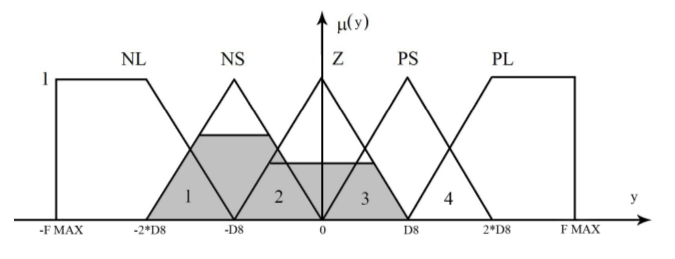
\includegraphics[width=0.6\textwidth]{./04-figuras/Maj2013_fuzzy_sets_output}
    \fonte{\cite{Maj2013}}
    \label{fig:Maj2013_fuzzy_sets_output}
\end{figure}

Os autores obtiveram sucesso no controle de estabilidade do \textit{drone}, mas somente utilizando um bloco integrador. Apesar de os reguladores e motores serem do mesmo tipo, algumas características deles são levemente diferentes. Como consequência, os motores não giram todos na mesma velocidade causando uma inclinação do quadrotor. A correção desta inclinação é possível com o uso do bloco integrador. Desta forma, foi observado que um controlador puramente fuzzy não é suficiente para lidar com esta situação. A solução encontrada foi, portanto, implementar um controlador híbrido, que se mostrou eficiente para tal propósito.

%06
%\cite{Coza2006}
\citeonline{Coza2006} propuseram um controlador fuzzy adaptativo para controlar a estabilidade de um quadricóptero \textit{Outdoor}. A escolha deste tipo de controlador se deu graças a inconvenientes apresentados por outros métodos. Controle adaptativo pode ser apropriado mas requer conhecimento aprofundado do tipo de não linearidades nas dinâmicas. Um SMC (\textit{Sliding Mode Control}\footnote{Controle de Deslizamento de Modo, tradução nossa}) pode ser apropriado mas pode causar vibração indesejada no sinal de controle. Controles por RNAs podem ser apropriados, mas requerem intenso esforço computacional para operar.

A abordagem utilizada em \cite{Coza2006} se baseia na ideia de que diferentes conjuntos de centros de decodificação são capazes de aproximar uniformemente a mesma função não linear. Desta forma, é usado treino supervisionado sobre os centros alternados: o erro do estado treina o centro de controle e a diferença na saída treina os centros alternados. A partir de simulações, mostrou-se que o resultado obtido foi um controle estável, computacionalmente eficiente e teoricamente robusto a perturbações. Entretanto, em uma das situações de simulações de perturbações por vento, o controlador teve de sacrificar a boa performance computacional para prevenir o desvio de centro. Ainda assim, foi mostrado que um modelo fuzzy adaptativo usando atualização de controle e centro pode ser usado para cada eixo de rotação: X, Y e Z. Para tanto, apenas quatro funções Gaussianas de pertinência fuzzy foram usadas para cada entrada de controle.

%10
%\cite{Rabhi2011}
Em \cite{Rabhi2011} uma outra abordagem é utilizada. Neste caso, os autores propuseram um controlador Fuzzy TSK (Takagi-Sugeno-Kang) para controlar a estabilidade de um quadrotor. O controlador foi modelado usando ferramentas matemáticas, mais especificamente a LMI (\textit{Linear Matrix Inequalities}\footnote{Desigualdades Matriciais Lineares}) e modelado empregando PDC (\textit{Parallel Distributed Compensation}\footnote{Compensação Paralela Distribuída}). O objetivo é projetar um controlador fuzzy realimentado para garantir a estabilidade do sistema com robustez. Simulações mostram que o controlador projetado garante, de fato, a estabilidade global do sistema em malha fechada.

%13
%\cite{Sheikhpour2013}
\citeonline{Sheikhpour2013} seguiram a mesma linha de \citeonline{Rabhi2011} e propuseram um controlador fuzzy TSK para estabilização de altura de um quadrotor. Mais uma vez, a técnica PDC foi utilizada para projetar o controlador de realimentação. Neste trabalho, entretanto, o controle de estabilidade deve se dar levando em conta especificações de performance como taxa de decaimento e restrições na entrada. Como ambas condições podem ser representadas por LMIs, elas também foram usadas neste caso, sendo mais complexas por lidar com as restrições dadas. Foi mostrado que simultaneamente à resolução das LMIs, foi projetado não apenas um controlador fuzzy estável mas também com inclusão de resposta de velocidade desejada e restrições na altitude de entrada no controlador. Os resultados obtidos em simulações mostram a viabilidade desta abordagem.

%16
%\cite{JavidiNiroumand2013}
\cite{JavidiNiroumand2013} propuseram uma forma alternativa de controlador também usando a lógica fuzzy. Na abordagem utilizada, primeiramente foi derivado um modelo dinâmico não linear de um quadrotor e então foi desenvolvido o controlador híbrido usando métodos de controle tradicionais e inteligentes para estabilização de dinâmicas rotacionais. A técnica IBS (\textit{Integral Backstepping}\footnote{Backstepping Integral, tradução nossa}) é um poderoso método de controle tradicional amplamente utilizado para tal tipo de sistema mas encontrar o coeficiente apropriado do algoritmo é um trabalho crítico. Neste caso, este problema foi resolvido usando um método de controle fuzzy. Foi mostrado nos resultados que o método IBS possui domínio de atração mais amplo em comparação a métodos de controle lineares como o PID e uma melhor convergência devido a condições iniciais rígidas. Foi mostrado ainda que ambos controladores IBS e Fuzzy IBS foram capazes de controlar o sistema de forma apropriada. Entretanto, o controlador FIBS (\textit{Fuzzy Integral Backstepping}\footnote{Backstepping Integral Fuzzy, tradução nossa}) obteve resultados levemente superiores ao IBS além de ter apresentado benefícios como uma melhor rejeição a perturbações e melhor robustez.

%20
%\cite{Ariffanan2014}
Em \cite{Ariffanan2014}, foi proposto um controlador FSBC (\textit{Fuzzy Supervisory Backstepping Controller}\footnote{Controlador por Backstepping Fuzzy Supervisionado, tradução nossa}). O controlador projetado consiste em controlador de \textit{backstepping} que pode selecionar automaticamente seus parâmetros \textit{on line} por um mecanismo de supervisão fuzzy. O critério de estabilidade para a estabilização do quadrotor é provada pelo teorema de Lyapunov. Extensivas simulações mostram a eficácia desta abordagem, apontando que uma alta precisão no transiente e no tempo de controle foram alcançados. Além disto, os resultados indicam que a técnica proposta pode estabilizar quadrotores UAV com melhor performance se comparado a técnicas de estabilização lineares.

%24
%\cite{Benavidez2014}
Em \cite{Benavidez2014} foi implementado um controlador fuzzy para controlar um quadrotor do modelo AR Drone 2.0 para trabalhar em conjunto com um UGV (\textit{Unmanned Ground Vehicle}\footnote{Veículos Terrestres não Tripulados, tradução nossa}). Este seria o caso, por exemplo, de o UGV prover espaço para aterrissagem, recarga de bateria e/ou serviços físicos ao UAV, que é limitado em termos de bateria. Desta forma, este trabalho lida com um UAV rastreando e aterrissando sobre um UGV.

O controlador foi projetado baseado em diferentes questões. O que se deseja controlar é a altitude do drone e esta informação pode ser obtida a partir do sonar embutido no modelo.

A principal função do controlador será estabilizar o \textit{drone} em altitude e, ao mesmo tempo, alcançar o ângulo de orientação desejado, de forma a permitir que ele alcance o UGV com sucesso. Para tanto, o \textit{drone} precisa de velocidade de translação ao longo to eixo y local enquanto rotaciona em torno do seu eixo z para reduzir o ângulo de orientação. Sobretudo, o objetivo é obter a mesma orientação em ambos UAV e UGV. Com a mesma orientação, o UAV pode se aproximar do UGV para operações de aterrissagem. Para se aproximar do UGV, uma vez orientado, o quadricóptero deve transladar ao longo do seu eixo x a fim de chegar próximo o suficiente para usar a câmera inferior possibilitando a detecção do bloco de aterrissagem.

A modelagem usando lógica Fuzzy aplicada ao controle de altitude se deu utilizando cinco diferentes termos linguísticos. As regras utilizadas são mostradas no \autoref{qua:Benavidez2014_table_rules_inference}.

\begin{quadro}[!htb]
    \centering
    \caption{Regras de inferência fuzzy usadas em \cite{Benavidez2014}\label{qua:Benavidez2014_table_rules_inference}}
    \begin{tabular}{|c|c|c|c|}
        \hline
        \textbf{Input} & 
        \textbf{Input MF} &
        \textbf{Output} &
        \textbf{Output MF} \\
        \hline
            sonar\textunderscore reading &
            too\textunderscore low &
            cmd\textunderscore vel\textunderscore gaz &
            large\textunderscore increase\textunderscore velocity \\
        \hline
            sonar\textunderscore reading &
            a\textunderscore little\textunderscore low &
            cmd\textunderscore vel\textunderscore gaz &
            small\textunderscore increase\textunderscore velocity \\
        \hline
            sonar\textunderscore reading &
            on\textunderscore target &
            cmd\textunderscore vel\textunderscore gaz &
            no\textunderscore change \\
        \hline
            sonar\textunderscore reading &
            a\textunderscore little\textunderscore high &
            cmd\textunderscore vel\textunderscore gaz &
            small\textunderscore decrease\textunderscore velocity \\
        \hline
            sonar\textunderscore reading &
            too\textunderscore high &
            cmd\textunderscore vel\textunderscore gaz &
            large\textunderscore decrease\textunderscore velocity \\
        \hline
    \end{tabular}
    \fonte{Adaptado de \citeonline{Benavidez2014}}
\end{quadro}


Como se pode ver, a entrada do sistema é a leitura do sonar, e ela está associada a cinco funções de pertinência: muito baixo, baixo, no alvo, alto e muito alto. A saída do sistema é o comando de velocidade de giro em torno do eixo z. Para cada um dos valores de entrada, a saída assume as seguintes funções de pertinência respectivamente: grande aumento na velocidade, pequeno aumento na velocidade, sem mudanças na velocidade, pequena redução na velocidade e, por fim, grande redução na velocidade. Todos os termos linguísticos foram modelados a partir de ondas gaussianas dentro dos limites de operação.

Os detalhes acerca do controle de ajuste de ângulo entre o UAV e o UGV usados não serão citados por não possuírem relação direta com este trabalho. O controle de estabilidade em altitude implementado se mostrou eficiente e os autores propuseram, para trabalhos futuros, o uso de um controlador neuro-fuzzy com treinamento supervisionado e \textit{data mining} para obter as entradas, regras e termos linguísticos ótimos baseados em histórico prévio de dados de voo.
%
%
%\subsection{Métodos de Controle Híbrido de Helicópteros Quadrotores}
%\label{sec:trab-rel-quadrotores-sub-hib}
%
%19
%\cite{Gao2014Stability}
Em \cite{Gao2014Stability}, é proposto um outro tipo de controlador híbrido. Neste caso, o controle é feito a partir de um sistema composto por dois controladores independentes: um controlador \textit{Backstepping} e um segundo controlador Fuzzy PID, que alia a lógica fuzzy a um controlador PID. Quando o quadrotor voa em boas condições, o controle de estabilidade é assumido pelo controlador \textit{Backstepping}. Quando o quadrotor encontra vento ou outro fator de perturbação durante o voo, o controlador Fuzzy PID é usado para estabilizá-lo.

O controlador Fuzzy PID é um controlador PID que emprega o Sistema de Inteferência Fuzzy (FIS) para ajustar os parâmetros $K_p$, $K_i$, $K_d$, ganhos proporcional, integral e diferencial respectivamente. A \autoref{fig:Gao2014Stability_block_diagram} mostra o diagrama de blocos representando o controlador Fuzzy PID.

\begin{figure}[!htb]
    \centering
    \caption{Diagrama de blocos do controlador híbrido usando em \cite{Gao2014Stability}}
    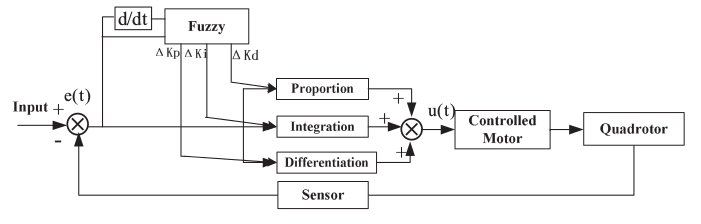
\includegraphics[width=0.9\textwidth]{./04-figuras/Gao2014Stability_block_diagram}
    \fonte{\citeonline{Gao2014Stability}}
    \label{fig:Gao2014Stability_block_diagram}
\end{figure}

Em relação à estrutura fuzzy, há duas entradas para a inferência fuzzy: o erro e a derivada do erro. São três saídas, cada uma sendo um parâmetro do controlador PID $\Delta kp$, $\Delta ki$ e $\Delta kd$. O universo de discurso foi normalizado e dividido em sete subconjuntos fuzzy. Os termos linguísticos foram definidos da seguinte forma: NB, negativo grande; NM, negativo médio; NS, negativo pequeno; ZO, aproximadamente zero; PS, positivo pequeno; PM, positivo médio; e PB, positivo grande. Os conjuntos fuzzy para cada variável de entrada consistem de sete variáveis linguísticas: $e$ = \{NB, NM, NS, ZO, PS, PM, PB\}, $e_c$ = \{NB, NM, NS, ZO, PS, PM, PB\}. As variáveis linguísticas das saídas são atribuídas da seguinte forma: $\Delta kp$ = \{ZO, PS, PM, PB\}, $\Delta ki$ = \{ZO, PS, PM, PB\}, $\Delta kp$ = \{ZO, PS, PM, PB\}. As regras de inferência Fuzzy para as variáveis de saída $\Delta kp$, $\Delta ki$ e $\Delta kd$ são mostradas nos Quadros \ref{qua:Gao2014Stability_table_rules_inference_kp}, \ref{qua:Gao2014Stability_table_rules_inference_ki} e \ref{qua:Gao2014Stability_table_rules_inference_kd} respectivamente.

\begin{quadro}[!htb]
    \centering
    \caption{Regras de inferência fuzzy usadas em \cite{Gao2014Stability} para a variável $\Delta K_p$\label{qua:Gao2014Stability_table_rules_inference_kp}}
    \begin{tabular}{c|c|c|c|c|c|c|c|}
        \cline{2-8}
        & \multicolumn{7}{c|}{\textbf{$\Delta E_c$}} \\
        
        %cabeçalho
        \hline
        \multicolumn{1}{ |c| }{\textbf{E}} & 
                            \textbf{NB} &
                            \textbf{NN} & 
                            \textbf{NS} & 
                            \textbf{ZO} & 
                            \textbf{PS} & 
                            \textbf{PM} & 
                            \textbf{PB} \\
        \hline
        %NB OK
        \multicolumn{1}{ |c| }{\textbf{NB}} & 
                            PB &
                            PM &
                            ZO &
                            ZO &
                            ZO &
                            PM &
                            PB \\
        \hline
        %NM OK
        \multicolumn{1}{ |c| }{\textbf{NM}} & 
                            PB &
                            PM &
                            ZO &
                            ZO &
                            ZO &
                            PM &
                            PB \\
        \hline
        %NS OK
        \multicolumn{1}{ |c| }{\textbf{NS}} & 
                            PB &
                            PB &
                            PS &
                            ZO &
                            PS &
                            PB &
                            PB \\
        \hline
        %ZO OK
        \multicolumn{1}{ |c| }{\textbf{ZO}} & 
                            PB &
                            PB &
                            PS &
                            ZO &
                            PS &
                            PB &
                            PB \\
        \hline
        %PS OK
        \multicolumn{1}{ |c| }{\textbf{PS}} & 
                            PB &
                            PB &
                            PS &
                            ZO &
                            PS &
                            PB &
                            PB \\
        \hline
        %PM OK
        \multicolumn{1}{ |c| }{\textbf{PM}} & 
                            PB &
                            PM &
                            ZO &
                            ZO &
                            ZO &
                            PM &
                            PB \\
        \hline
        %PB OK
        \multicolumn{1}{ |c| }{\textbf{PB}} & 
                            PB &
                            PM &
                            ZO &
                            ZO &
                            ZO &
                            PM &
                            PB \\
        \hline

        % \multicolumn{1}{ |c| }{\textbf{NB}} & 
        %                     PB/ZO/PB &
        %                     PB/ZO/PB &
        %                     PB/ZO/PB &
        %                     PB/ZO/PB &
        %                     PB/ZO/PB &
        %                     PB/ZO/PB &
        %                     PB/ZO/PB \\
        % \hline

    \end{tabular}
    \fonte{Adaptado de \citeonline{Gao2014Stability}}
\end{quadro}







\begin{quadro}[!htb]
    \centering
    \caption{Regras de inferência fuzzy usadas em \cite{Gao2014Stability} para a variável $\Delta K_i$\label{qua:Gao2014Stability_table_rules_inference_ki}}
    \begin{tabular}{c|c|c|c|c|c|c|c|}
        \cline{2-8}
        & \multicolumn{7}{c|}{\textbf{$\Delta E_c$}} \\
        
        %cabeçalho
        \hline
        \multicolumn{1}{ |c| }{\textbf{E}} & 
                            \textbf{NB} &
                            \textbf{NN} & 
                            \textbf{NS} & 
                            \textbf{ZO} & 
                            \textbf{PS} & 
                            \textbf{PM} & 
                            \textbf{PB} \\
        \hline
        %NB OK
        \multicolumn{1}{ |c| }{\textbf{NB}} & 
                            ZO &
                            ZO &
                            ZO &
                            PS &
                            ZO &
                            ZO &
                            ZO \\
        \hline
        %NM OK
        \multicolumn{1}{ |c| }{\textbf{NM}} & 
                            ZO &
                            ZO &
                            ZO &
                            PS &
                            ZO &
                            ZO &
                            ZO \\
        \hline
        %NS OK
        \multicolumn{1}{ |c| }{\textbf{NS}} & 
                            ZO &
                            ZO &
                            PS &
                            PS &
                            PS &
                            ZO &
                            ZO \\
        \hline
        %ZO OK
        \multicolumn{1}{ |c| }{\textbf{ZO}} & 
                            ZO &
                            ZO &
                            PS &
                            PS &
                            PS &
                            ZO &
                            ZO \\
        \hline
        %PS OK
        \multicolumn{1}{ |c| }{\textbf{PS}} & 
                            ZO &
                            ZO &
                            PS &
                            PS &
                            PS &
                            ZO &
                            ZO \\
        \hline
        %PM OK
        \multicolumn{1}{ |c| }{\textbf{PM}} & 
                            ZO &
                            ZO &
                            ZO &
                            PS &
                            ZO &
                            ZO &
                            ZO \\
        \hline
        %PB OK
        \multicolumn{1}{ |c| }{\textbf{PB}} & 
                            ZO &
                            ZO &
                            ZO &
                            PS &
                            ZO &
                            ZO &
                            ZO \\
        \hline

        % \multicolumn{1}{ |c| }{\textbf{NB}} & 
        %                     PB/ZO/PB &
        %                     PB/ZO/PB &
        %                     PB/ZO/PB &
        %                     PB/ZO/PB &
        %                     PB/ZO/PB &
        %                     PB/ZO/PB &
        %                     PB/ZO/PB \\
        % \hline

    \end{tabular}
    \fonte{Adaptado de \citeonline{Gao2014Stability}}
\end{quadro}







\begin{quadro}[!htb]
    \centering
    \caption{Regras de inferência fuzzy usadas em \cite{Gao2014Stability} para a variável $\Delta K_d$\label{qua:Gao2014Stability_table_rules_inference_kd}}
    \begin{tabular}{c|c|c|c|c|c|c|c|}
        \cline{2-8}
        & \multicolumn{7}{c|}{\textbf{$\Delta E_c$}} \\
        
        %cabeçalho
        \hline
        \multicolumn{1}{ |c| }{\textbf{E}} & 
                            \textbf{NB} &
                            \textbf{NN} & 
                            \textbf{NS} & 
                            \textbf{ZO} & 
                            \textbf{PS} & 
                            \textbf{PM} & 
                            \textbf{PB} \\
        \hline
        %NB OK
        \multicolumn{1}{ |c| }{\textbf{NB}} & 
                            PB &
                            PB &
                            PM &
                            PS &
                            PM &
                            PB &
                            PB \\
        \hline
        %NM OK
        \multicolumn{1}{ |c| }{\textbf{NM}} & 
                            PB &
                            PB &
                            PM &
                            PS &
                            PM &
                            PB &
                            PB \\
        \hline
        %NS OK
        \multicolumn{1}{ |c| }{\textbf{NS}} & 
                            PB &
                            PM &
                            PS &
                            ZO &
                            PS &
                            PM &
                            PB \\
        \hline
        %ZO OK
        \multicolumn{1}{ |c| }{\textbf{ZO}} & 
                            PB &
                            PM &
                            PS &
                            ZO &
                            PS &
                            PM &
                            PB \\
        \hline
        %PS OK
        \multicolumn{1}{ |c| }{\textbf{PS}} & 
                            PB &
                            PM &
                            PS &
                            ZO &
                            PS &
                            PM &
                            PB \\
        \hline
        %PM OK
        \multicolumn{1}{ |c| }{\textbf{PM}} & 
                            PB &
                            PB &
                            PM &
                            ZO &
                            PM &
                            PB &
                            PB \\
        \hline
        %PB OK
        \multicolumn{1}{ |c| }{\textbf{PB}} & 
                            PB &
                            PB &
                            PM &
                            PS &
                            PM &
                            PB &
                            PB \\
        \hline

        % \multicolumn{1}{ |c| }{\textbf{NB}} & 
        %                     PB/ZO/PB &
        %                     PB/ZO/PB &
        %                     PB/ZO/PB &
        %                     PB/ZO/PB &
        %                     PB/ZO/PB &
        %                     PB/ZO/PB &
        %                     PB/ZO/PB \\
        % \hline

    \end{tabular}
    \fonte{Adaptado de \citeonline{Gao2014Stability}}
\end{quadro}







O controlador proposto alcançou sucesso nos testes realizados, mostrando permitir completar a trajetória sem que perturbações afetem a precisão de controle. O Sistema de Inferência Fuzzy se mostrou eficiente para ajustar os ganhos do controlador PID de forma a possibilitar o controle eficiente do quadrotor.

%28
%\cite{Gao2014Precision}
Em outro trabalho, os mesmos autores implementaram um outro controlador híbrido. Em \cite{Gao2014Precision}, foi proposto um controlador Fuzzy PD. Além disto, neste trabalho, são comparadas as performances de três controladores diferentes: PID, Fuzzy PD e \textit{Backstepping}. Mais uma vez, aqui o controlador fuzzy tem como função ajustar os parâmetros do controlador PD: $\Delta K_p$ e $\Delta K_d$.

A \autoref{fig:Gao2014Precision_block_diagram} mostra o diagrama de blocos do controlador neste caso. Como se pode ver, o diagrama mostra o controlador Fuzzy PD e um controlador PID.

\begin{figure}[!htb]
    \centering
    \caption{Diagrama de blocos do controlador híbrido usando em \cite{Gao2014Precision}}
    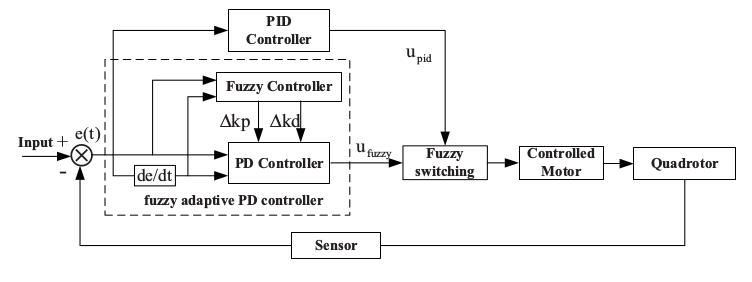
\includegraphics[width=0.9\textwidth]{./04-figuras/Gao2014Precision_block_diagram}
    \fonte{\citeonline{Gao2014Precision}}
    \label{fig:Gao2014Precision_block_diagram}
\end{figure}

Em relação à estrutura fuzzy, mais uma vez aqui há duas entradas para a inferência: o erro, sua derivada e os conjuntos fuzzy para cada uma delas consistem de sete variáveis linguísticas: $e$ = \{NB, NM, NS, ZO, PS, PM, PB\}, $e_c$ = \{NB, NM, NS, ZO, PS, PM, PB\}. A variável de saída do sistema Fuzzy PD é apenas uma: $U_{fuzzy}$ = \{ZO, PS, PM, PB\}. O \autoref{qua:Gao2014Precision_table_rules_inference} mostra as regras definidas para o sistema de inferência fuzzy.

\begin{quadro}[!htb]
    \centering
    \caption{Regras de inferência fuzzy usadas em \cite{Gao2014Precision}\label{qua:Gao2014Precision_table_rules_inference}}
    \begin{tabular}{c|c|c|c|c|c|c|c|}
        \cline{2-8}
        & \multicolumn{7}{c|}{\textbf{$\Delta E_c$}} \\
        
        %cabeçalho
        \hline
        \multicolumn{1}{ |c| }{\textbf{E}} & 
                            \textbf{NB} &
                            \textbf{NN} & 
                            \textbf{NS} & 
                            \textbf{ZO} & 
                            \textbf{PS} & 
                            \textbf{PM} & 
                            \textbf{PB} \\
        \hline
        %NB OK
        \multicolumn{1}{ |c| }{\textbf{NB}} & 
                            PB &
                            PM &
                            PM &
                            PS &
                            PM &
                            PM &
                            PB \\
        \hline
        %NM OK
        \multicolumn{1}{ |c| }{\textbf{NM}} & 
                            PB &
                            ZO &
                            ZO &
                            PS &
                            ZO &
                            ZO &
                            ZO \\
        \hline
        %NS OK
        \multicolumn{1}{ |c| }{\textbf{NS}} & 
                            ZO &
                            ZO &
                            PS &
                            ZO &
                            PM &
                            PB &
                            ZO \\
        \hline
        %ZO OK
        \multicolumn{1}{ |c| }{\textbf{ZO}} & 
                            PM &
                            PB &
                            PS &
                            ZO &
                            ZO &
                            PM &
                            PB \\
        \hline
        %PS OK
        \multicolumn{1}{ |c| }{\textbf{PS}} & 
                            PS &
                            PB &
                            PS &
                            PM &
                            PS &
                            ZO &
                            PB \\
        \hline
        %PM 
        \multicolumn{1}{ |c| }{\textbf{PM}} & 
                            PB &
                            ZO &
                            ZO &
                            PM &
                            ZO &
                            PM &
                            ZO \\
        \hline
        %PB 
        \multicolumn{1}{ |c| }{\textbf{PB}} & 
                            ZO &
                            PM &
                            PM &
                            ZO &
                            PM &
                            PM &
                            PM \\
        \hline
    \end{tabular}
    \fonte{Adaptado de \citeonline{Gao2014Precision}}
\end{quadro}







O controlador Fuzzy PD é adotado para garantir uma supressão rápida e com sobrelevação quando o desvio é grande. Já o controlador PID é adotado para eliminar o estado estacionário quando o desvio é pequeno.

A definição de qual dos controles irá atuar, depende do bloco \textit{Fuzzy switching}, que avalia os sinais $u_{pid}$ e $u_{fuzzy}$, e utiliza o mais apropriado entre eles. A regra utilizada é a seguinte: se $E(k)$ é $SE$ e $\Delta EC(k)$ é $S\Delta EC$ então $U$ é $U_{pid}$, senão $U$ é $U_{fuzzy}$, em que $U_{fuzzy}$ e $U_{pid}$ são as saídas dos controladores Fuzzy PD e PID respectivamente. $SE$ e $S\Delta EC$ são, respectivamente, funções de pertinência fuzzy das variáveis $E$ e $\Delta E_c$.

Nas simulações feitas, foram comparados três controladores diferentes: \textit{Backstepping}, PID e Fuzzy PD. Foi verificado que, embora o controlador \textit{Backstepping} seja pior que os outros dois, ele pode rapidamente suprimir o impacto de perturbações. Foi mostrado ainda que o controlador Fuzzy PD obteve o melhor resultado relacionado a rejeição de perturbações. O tempo de subida do controlador Fuzzy PD é ligeiramente menor nos eixos x e z mas um pouco maior no eixo y. Após numerosas simulações, verificou-se que o controlador proposto é, de fato, eficaz para manter a estabilidade de um helicóptero quadrotor.

%15
%\cite{Fatan2013}
\citeonline{Fatan2013} propuseram, para o controle de estabilidade de um \textit{drone}, um ANP (\textit{Adaptive Neuro PID Controller}\footnote{Controlador Neuro PID Adaptativo}), que na verdade não implementa de fato uma rede neural. O nome foi dado devido à similaridade de estrutura entre o controlador obtido e uma rede neural, em que o sistema atua, no treinamento, para ajustar os pesos das conexões. O controlador implementado utiliza outra técnica de IA: é utilizado um algoritmo genético para ajustar três pesos $w_1$, $w_2$ e $w_3$, responsáveis por ajustar os pesos $\Delta K_p$, $\Delta K_i$ e $\Delta K_d$ do controlador PID respectivamente.

A importante vantagem deste método é não precisar de análises matemáticas para cada situação de perturbação a ser enfrentada pelo \textit{drone} sendo ele próprio capaz de ajustar os pesos para que o controle seja efetivo em diferentes condições. Entretanto, não é garantido que os coeficientes apropriados sejam obtidos para todos os casos. Outro problema é a questão de o fator de aprendizagem utilizado no controlador ser crítica, uma vez que uma taxa muito baixa pode não levar a uma adaptação rápida o suficiente para garantir a estabilidade numa mudança de situação. Apesar das limitações, foi mostrado que o controlador ANP pode controlar o sistema na presença de ruídos e perturbações que mesmo o controlador PID com ganhos bem definidos não pode controlar bem.

%17
%\cite{Yacef2013}
Outras abordagens híbridas ainda foram adotadas para o projeto de controladores de estabilidade para \textit{drones}. Em \cite{Yacef2013}, foi proposto o uso do PSO para ajuste de um IBC. O método é usado para minimizar o erro quadrático (SE) de uma função de custo que quantifica a performance de todo o sistema. Resultados de numerosas simulações mostram a validação e as boas performances alcançadas pelo método proposto.

%18
%\cite{Boubertakh2013}
Em \cite{Boubertakh2013} é proposta uma ideia parecida: utilizar o algoritmo PSO para ajustar os pesos de quatro controladores PD, cada qual responsável por controlar um rotor. A ideia é usar o PSO para minimizar o SE da função de custo que quantifica o sistema, assim como visto em \cite{Yacef2013}. As simulações feitas mostraram a eficácia do controlador proposto.